\documentclass[10pt]{article}
\usepackage{latexsym}
\usepackage{natbib}
\usepackage{graphicx}
\usepackage{subfigure}
\usepackage{listings}
\usepackage{algorithm}
\usepackage{algpseudocode}

\title{Homework 1: Eigendigits}
\author{Shun Zhang}
\date{}

\begin{document}
\maketitle

\section{Introduction}

In this report, I applied principal components analysis on digits
classification problem.

In our example, the original figures are represented in
728-dimensional vectors. This is a comparatively high dimensional
representation. Distance of vectors in this space would be very large.
This fact is also known as ``curse of dimension''. It would be low
efficient to do learning in this high-dimensional space, so reduction
on dimension is necessary.

However, figures of digits should be easy to describe - they need far
less than 728 dimensions. The motivation is that we want use a basis
such that coordinates of the figures vary the most. This would be the
most expressive way in a limited dimension. We could look into the
covarance matrix of the data, and use its eigenvectors with maximum
eigenvalues.

\section{Algorithm}

Let a figure be in size of $n \times n$. Let $X$ be the matrix such
that each column of it is a datum, represented as an unrolled vector
of size of $n^2 \times 1$. Let there be $K$ samples. Then the
dimension of $X$ is $n^2 \times K$. The covarance of $X$ is defined
as,
$$Cov(X) = \mathrm{E}((X - \mathrm{E}(X))(X - \mathrm{E}(X))^T)$$
Let $A = X - \mathrm{E}(X)$. As $A$ is in $n^2 \times n^2$ dimension,
we don't want to find eigenspace for this directly. As we know,
$$A^TAx = \lambda x$$
$$AA^TAx = \lambda Ax$$
we can find eigenvectors of $A^TA$, and lefty multiply them with $A$
to get eigenvectors of $AA^T$.

\begin{figure}
\centering
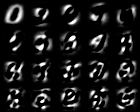
\includegraphics[]{eigen.png}
\caption{First 20 eigenvectors, using first 2000 training samples.
They are aligned from left to right and top to down. They become dark
after normalization. So in this figure, each value is multiplied by
10, i.e., each vector has norm of 100, instead of 1. }
\label{fig:eigen}
\end{figure}

Let $V$ be the set of the eigenvectors of $AA^T$, sorted descendingly
according to the eigenvalues. It's actually a set of basis we want to
use. The first 20 eigenvectors are shown in Figure~\ref{fig:eigen}.
Intuitively, eigenvectors with smaller eigenvalues care more about
details of the digits, while the ones with higher eigenvalues care
more about mean feautres of the digits.

If we call the basis we use as $B$ and the eigenspace as $E$. $V$
is a linear transformation from $E$ to $B$, usually represented as
$P_{BE}$ in the linear algebra literature. We also need $P_{EB}$,
which is defined as the inverse of $P_{BE}$. If $P_{BE}$ is
orthogonal, then $P_{EB} = P_{BE}^T$.  However, we don't have such
assumption. I used the left psudo-inverse of $P_{BE}$ to represent
$P_{EB}$.
$$P_{EB} = (P_{BE}^T P_{BE})^{-1} P_{BE}^T$$
Now, we can transform any vector in $B$ or $E$ basis to the other in
the following way.
$$[v]_B = P_{BE} [v]_E$$
$$[v]_E = P_{EB} [v]_B$$

\begin{figure}
\centering
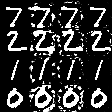
\includegraphics[]{test.png}
\caption{Reconstruction of digits. From left to right on each line,
there are original digits, digits constructed by first 100
eigenvectors, digits constructed by first 200 eigenvectors, and digits
constructed by first 600 eigenvectors. }
\label{fig:test}
\end{figure}

We can check how digits are "reconstructed" after maping from $B$ to
$E$ and then back to $B$. Figure~\ref{fig:test} shows the
reconstruction result, using 100, 200, and 600 eigenvectors
respectively. The more eigenvectors used, the more close it
reconstructed, and, as a cost, the heigher the dimension of $E$ is.

For classification, I transform the training set from $B$ to $E$ to
reduce its dimension. For a test sample, say $u$, I also transfermed
it to $E$ space, as $[v]_E$. I compute the distance of this to every
training sample. The k training samples with smallest distance are
selected. They majority of their labels is considered as the label of
this test datum. This is the idea of K-Nearest-Neighbors algorithm.

\section{Experiments}

%hw1Classify(n, 1000, 200, 1)
\begin{figure}
\centering
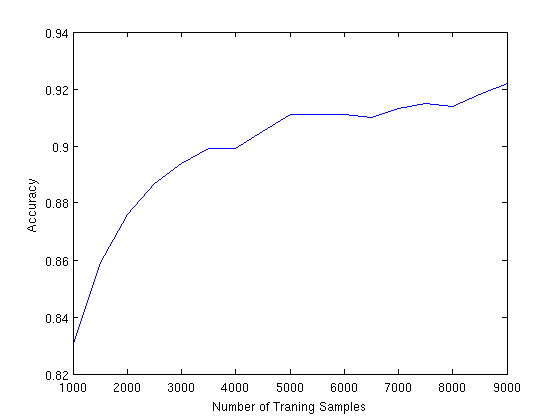
\includegraphics[width=0.5\columnwidth]{diffDataSet.png}
\caption{Comparison on using different number of training samples.
Testing on first 1000 testing set. Using first 200 eigen-vectors. K
for K-nearest-neighbors is 1.}
\label{fig:dataset}
\end{figure}

The first experiment tests the learning performance on different size
of data, shown in Figure~\ref{fig:dataset}. It's not surprising that
the more training data provided, the better accuracy can be achieved.

\begin{figure}
\centering
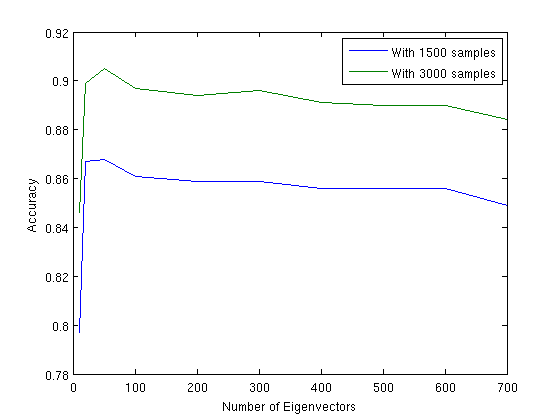
\includegraphics[width=0.5\columnwidth]{diffEVector.png}
\caption{Comparison on using different number of eigenvectors.
Testing on first 1000 testing set. Using first 1500 and 3000 training
samples for each line.  K for K-nearest-neighbors is 1.}
\label{fig:evec}
\end{figure}

The second experiment tests the learning performance on different set
of eigenvectors, shown in Figure~\ref{fig:evec}. Here is some
interesting observation. When too few eigenvectors are used, which
means $E$ has very small dimensions, the accuracy is low. This is
because vectors in $E$ are not expressive enough. However, when there
are too many eigenvectors provided, the learning performance would go
worse, as it's hard to learn in a high dimensional space.
Figure~\ref{fig:evec} shows that 50-100 eigenvectors have the best
performance, when the training set is fixed.

\begin{figure}
\centering
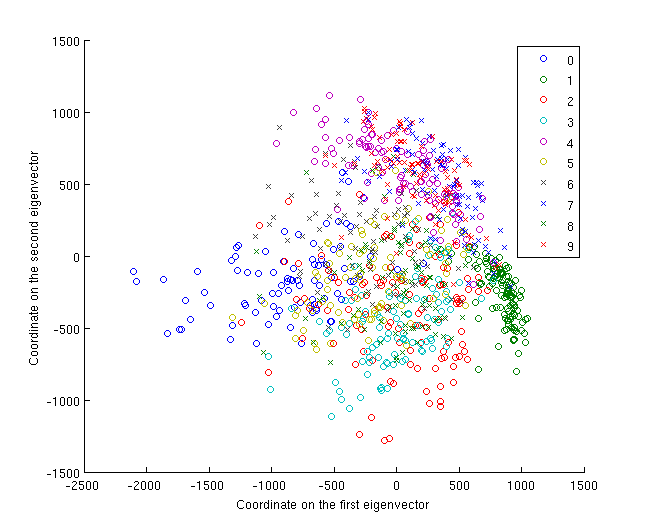
\includegraphics[width=0.5\columnwidth]{twod_digit.png}
\caption{Data coordinates on first two basis in $E$ space.  Using
first 5000 training samples. Testing on first 1000 testing samples.}
\label{fig:twod}
\end{figure}

Figure~\ref{fig:twod} shows the coordinates of data in $E$ basis, but
only on first two eigenvectors. They should spread the most on the
first basis, which is the horizontal axis, and less, but still much,
on the second basis, which is the verticle axis.

They have some clustering performance, while not disjunct. This is
because we didn't take labels into consideration when designing the
$E$ basis. $E$ basis makes data representation more efficient, but
doesn't help to separate data from different labels. The performance
of clustering in the figure is caused by the nature of difference
looking of figures.

\section{Conclusion}

In this assignment, I implemented principal components analysis to
classify digits in the eigenspace of the covariance matrix of the
data. This reduces the dimension of the data, with the least
information loss. This also works for compression purpose. However, I
believe that $E$ could be more carefully selected, which makes data in
different classes more separable for classification purpose.

\end{document}
